% https://tex.stackexchange.com/a/447784/173708

\documentclass[tikz, border=5pt]{standalone}

\usepackage{tikz}
\usepackage{lipsum}

\begin{document}
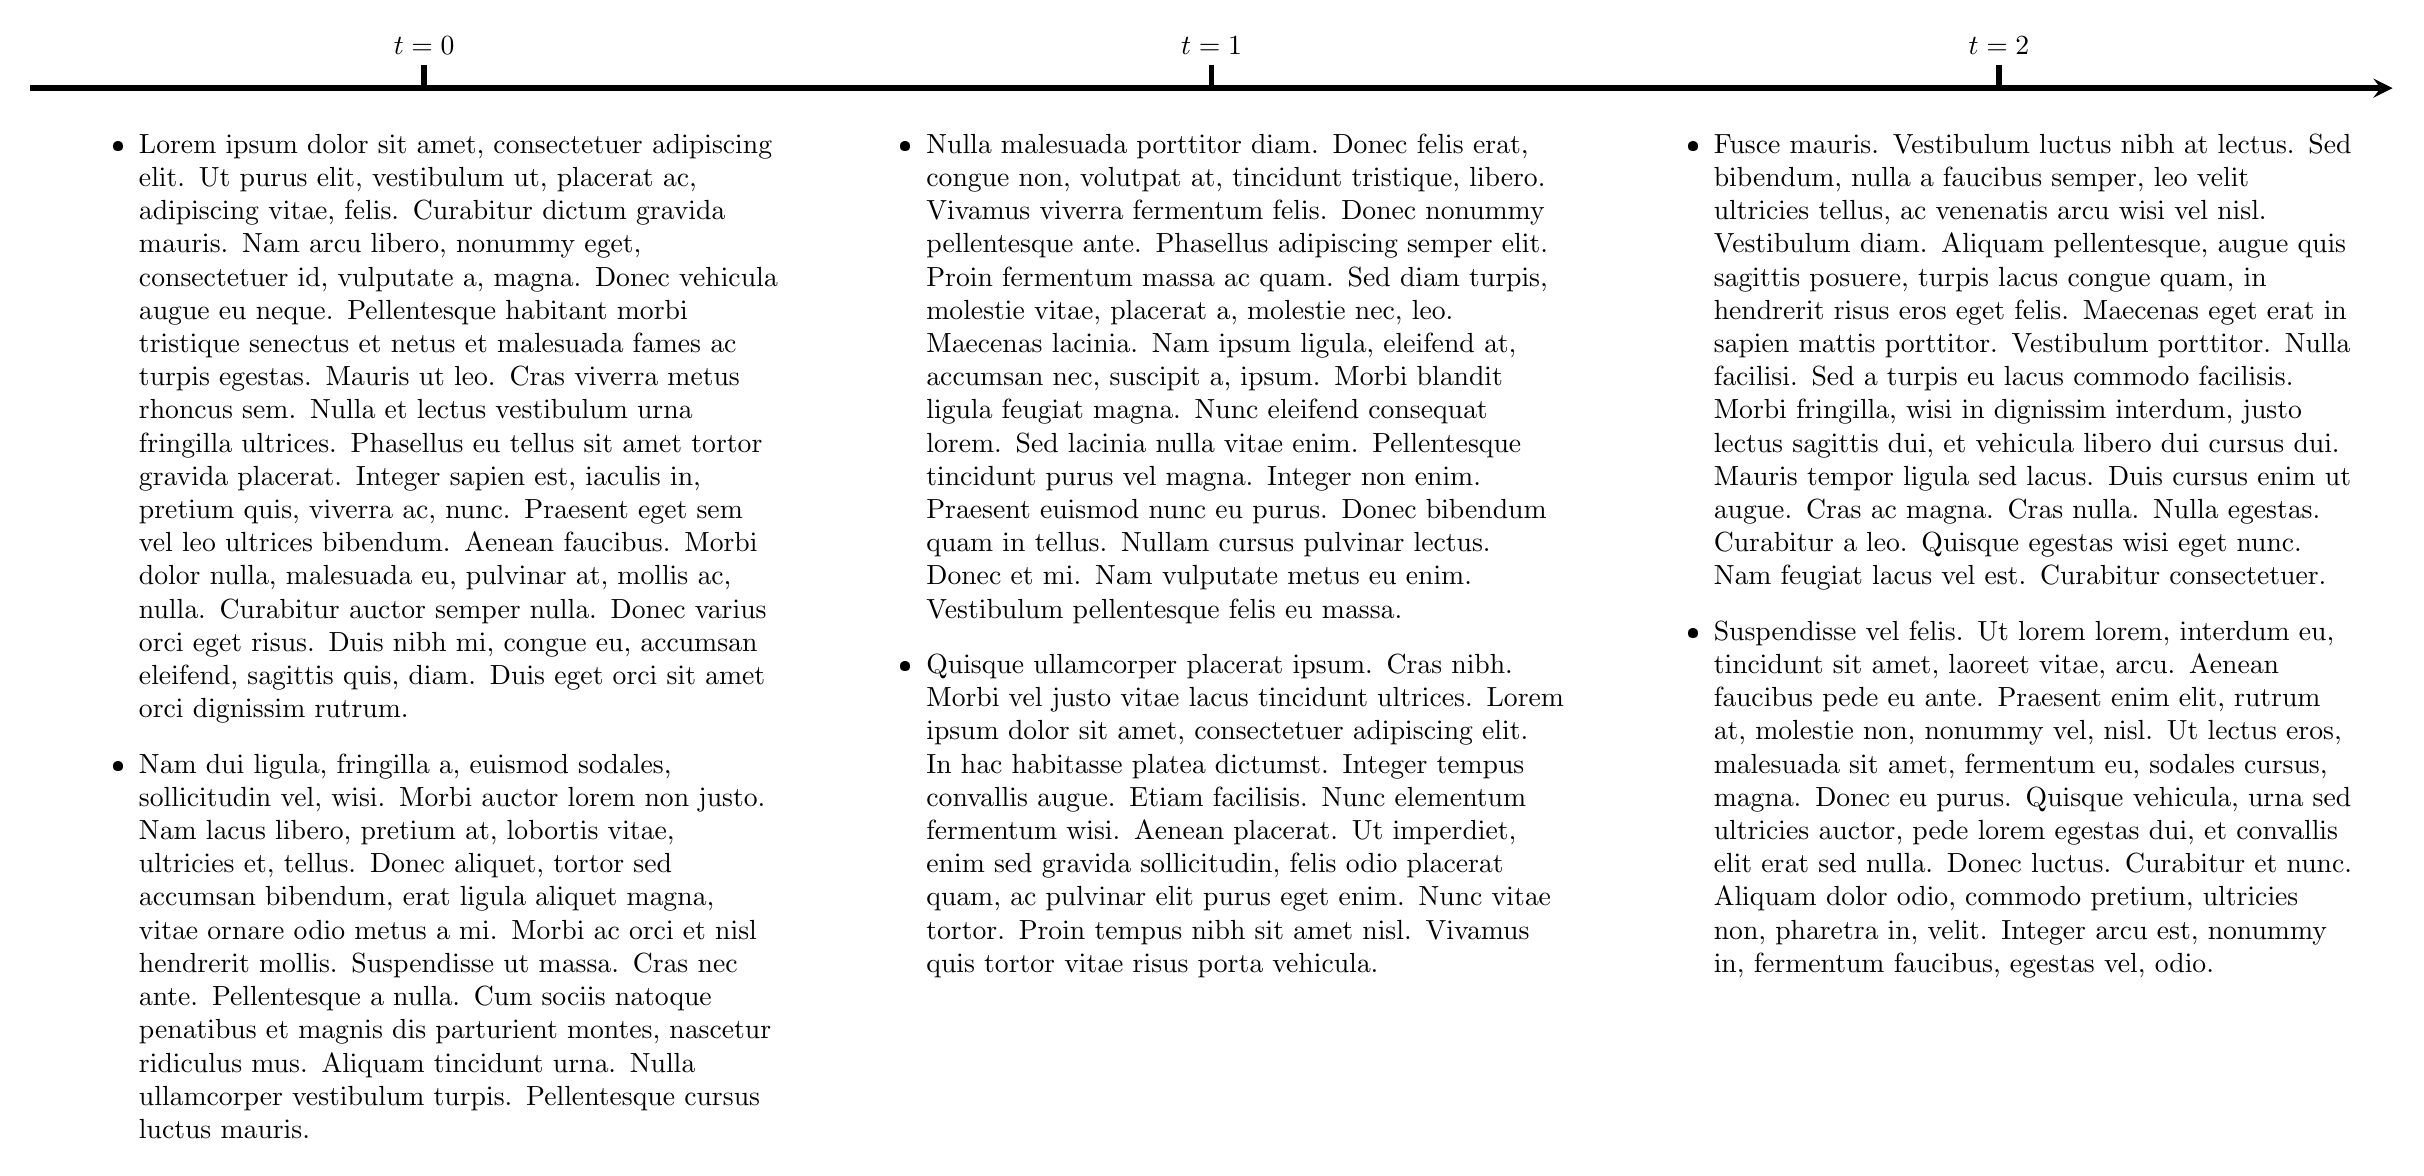
\begin{tikzpicture}
	\usetikzlibrary{calc}
	
	% draw arrow
	\coordinate (start) at (-4,0);
	\coordinate (end) at (26,0);
	\draw [line width=2pt, -stealth] (start) -- (end);
	
	% You can use `foreach` to improve the following codes
	\coordinate (s0) at (1,0);
	\coordinate (t0) at ($(s0)+(0,0.3)$);
	\coordinate (s1) at (11,0);
	\coordinate (t1) at ($(s1)+(0,0.3)$);
	\coordinate (s2) at (21,0);
	\coordinate (t2) at ($(s2)+(0,0.3)$);
	
	% draw ticks
	\draw [line width=2pt] (s0) -- (t0);
	\node [anchor=south] at (t0.north) {$t=0$};
	
	\draw [line width=2pt] (t1) -- (s1);
	\node [anchor=south] at (t1.north) {$t=1$};
	
	\draw [line width=2pt] (t2) -- (s2);
	\node [anchor=south] at (t2.north) {$t=2$};
	
	% add texts
	\node [anchor=north, align=left, text width=9cm] at (s0.south) {
	\begin{itemize}
	\item \lipsum[1]
	\item \lipsum[2]
	\end{itemize}
	};
	
	\node [anchor=north, align=left, text width=9cm] at (s1.south) {
	\begin{itemize}
	\item \lipsum[3]
	\item \lipsum[4]
	\end{itemize}
	};
	
	\node [anchor=north, align=left, text width=9cm] at (s2.south) {
	\begin{itemize}
	\item \lipsum[5]
	\item \lipsum[6]
	\end{itemize}
	};

\end{tikzpicture}
\end{document}